\documentclass[12pt,a4paper,utf8x, combine]{report}
\usepackage [english,frenchb]{babel} 
\usepackage{comment}

% Pour pouvoir utiliser  les accents
%\usepackage[combine]{ucs}
\usepackage{ucs}
\usepackage[utf8x]{inputenc}
\usepackage[T1]{fontenc}
\usepackage{textcomp, lmodern}
\usepackage[textwidth=7.10in]{geometry}

% Pour pouvoir inclure des images
\usepackage{float}
\usepackage{graphicx}
\usepackage{pdfpages}
\usepackage{filecontents}



% On définit le chemin par défaut des images 
\graphicspath{{images/}}
\usepackage[margin=10pt,font=small,labelfont=bf]{caption}

\usepackage[colorlinks = true, linkcolor = blue, urlcolor  = blue, citecolor = blue, anchorcolor = blue, unicode]{hyperref}% Pour avoir de belles urls
\usepackage {geometry}

% Pour mettre du code source
\usepackage {listings}
% Pour pouvoir passer en paysage
\usepackage{lscape}
\usepackage[compact]{titlesec}
\titlespacing{\chapter}{0pt}{-50pt}{240pt}
\titlespacing{\section}{0pt}{0pt}{0pt}
\titlespacing{\subsection}{20pt}{0pt}{0pt}
% Pour pouvoir faire plusieurs colonnes
\usepackage {multicol}
% Pour créer un index
\usepackage{makeidx}
\usepackage{lastpage}
\usepackage{amsmath}
\usepackage{array}
\makeindex

% Pour les entetes de page
\usepackage{fancyhdr}
\pagestyle{fancy}
\renewcommand{\chaptermark}[1]{\markboth{#1}{}}
\fancyhf{}
%\fancyheadoffset{\textwidth}

\fancyhead[L]{
\includegraphics[width=1.8cm]{deltacad.png}}
\fancyhead[R]{
\includegraphics[width=3cm]{utc.jpg}}
\fancyhead[C]{Rapport de stage TN10 - Jonathan DEKHTIAR\\}
%\fancyfoot[C]{\chaptername~\thechapter\\}
\fancyfoot[C]{\leftmark\\}
\fancyfoot[R]{Page : \thepage /\pageref*{LastPage}\\}

\fancypagestyle{plain}

\setlength\headheight{3cm} 

% Pour l'interligne de 1.5
%\usepackage {setspace}
% Pour les marges de la page
\geometry{a4paper, top=2.5cm, bottom=2.5cm, left=1.5cm, right=1.5cm, marginparwidth=1.2cm}

\parskip=20pt %% distance entre § (paragraphe)
\sloppy %% respecter toujours la marge de droite 

% Pour les pénalités :
\interfootnotelinepenalty=150 %note de bas de page

\widowpenalty=10000 % empeche au maximum la coupure avant la derniere ligne
\clubpenalty=10000  % empeche au maximum la coupure apres la premiere ligne
\raggedbottom   


%Pour la longueur de l'indentation des paragraphes
\setlength{\parindent}{0cm}

\begingroup
\makeatletter
% Redefine the \chapter* header macro to remove vertical space
\def\@makeschapterhead#1{%
  %\vspace*{50\p@}% Remove the vertical space
  {\parindent \z@ \raggedright
    \normalfont
    \interlinepenalty\@M
    \Huge \bfseries  #1\par\nobreak
    \vskip 1\p@
  }}
\def\@makechapterhead#1{%
  %\vspace*{50\p@}% Remove the vertical space
  {\parindent \z@ \raggedright
    \normalfont
    \interlinepenalty\@M
    \Huge \bfseries  #1\par\nobreak
    \vskip 1\p@
  }}
  
\makeatother

\bibliographystyle{IEEEtran}

\begin{document}

\makeatletter
\renewcommand{\@chapapp}{}% Not necessary...
\newenvironment{chapquote}[2][2em]
  {\setlength{\@tempdima}{#1}%
   \def\chapquote@author{#2}%
   \parshape 1 \@tempdima \dimexpr\textwidth-2\@tempdima\relax%
   \itshape}
  {\par\normalfont\hfill--\ \chapquote@author\hspace*{\@tempdima}\par\bigskip}
\makeatother


\includepdf[pages={1}]{couverture.pdf}
\input{remerciements}

\tableofcontents
\listoffigures
\clearpage

% Pour avoir un interligne de 1,5
%\begin{onehalfspace}

\chapter*{Introduction}
\markboth{Introduction}{}
\addcontentsline{toc}{chapter}{Introduction}

Dans le cadre de mes études en \emph{Génie Informatique, filière Fouille de Données (FDD)} à l'\textbf{Université de Technologie de Compiègne} (\url{http://www.utc.fr}), j'ai réalisé un stage Ingénieur de 6 mois dans l'entreprise DeltaCAD, spécialisée en informatique scientifique. 


Mon stage s'insère dans le cadre du projet de recherche, subventionné par l'ANR, METIS \\(\url{http://metis.deltacad.fr/}).

Au cours de mon stage, j'ai pu prendre part aux réunions de projet avec l'ensemble des partenaires académiques et industriels afin d'y présenter mes travaux.

L'objectif principal de ce stage fut de créer un "\textit{plugin de signature}" pour le logiciel METIS. Ce dernier devrait pouvoir signer une photo de pièce mécanique, et dans un deuxième temps être capable de comparer les signatures entres-elles.

Afin de mener cet objectif à bien, le stage fut composé de \textbf{différentes parties}.

Dans un premier temps, il fut primordial de réaliser une brève étude de l'\textit{état de l'art} associé au domaine de la rétro-conception de grands ensembles mécaniques.
Ensuite nous avons réorienté notre étude vers les méthodes existantes dans la littérature scientifique concernant la reconnaissance de forme ("\textit{Shape Matching}" et "\textit{Computer Vision}").

Nous avons pu identifier une méthode de mise en correspondance des formes grâce à l'utilisation de l'axe Median de Blum ou Squelette d'une Pièce. Cette méthode utilise également le concept de Shock Graph [K. Siddiqi et al]~\cite{Siddiqi1999}

Nous avons donc orienté mon travail sur la reprise du démonstrateur fonctionnel, mis en avant par [D. Macrini et al]~\cite{Macrini2002}, avec un objectif d'industrialisation du processus tout en apportant une vision orientée "\textit{grand volume de données}" au projet.
Dans un second temps il s'agira d'améliorer le résultat de l'algorithme de comparaison des \textit{ShockGraphs} et d'y adjoindre une fonctionnalité de préfiltrage des Graphs selon le contexte mécanique dans lequel on se place.

Finalement nous avons porté la solution vers le Cloud Amazon AWS, \url{http://aws.amazon.com/fr/}, afin d'assurer la fléxibilité en terme de stockage et puissance de calcul.

%\clearpage

\chapter{Présentation de l'entreprise}

\section{DeltaCAD, une entreprise d'informatique scientifique}

\subsection{Présentation de l'entreprise}

\textbf{DeltaCAD} est une société d'ingénierie spécialisée en CAO/Simulation et en informatique scientifique, créée en 1994.

Ses ingénieurs ont une expérience de plus de 20 ans dans ce domaine. Grâce à ses compétences reconnues par le marché, elle propose des services et des logiciels pour aider ses clients à concevoir, dimensionner, optimiser leurs produits, systèmes et procédés de fabrication.

L'offre de \textbf{DeltaCAD} est orientée vers les entreprises à fort potentiel technologique dans les secteurs:\\
\begin{itemize}
  \item Automobile
  \item Électronique
  \item Mécanique
  \item Énergie
  \item Aéronautique
  \item Génie Civil
  \item Édition de Logiciels
\end{itemize}
\vspace{5mm}

\textbf{DeltaCAD} propose, en outre, à ses clients et partenaires industriels :\\
\begin{itemize}
  \item Des services d'études, de conseil, de développement de logiciels et de gestion globale de logiciels spécifiques
  \item Des produits logiciels dans le domaine de la géométrie, du maillage et du transfert d'informations entre logiciels de modélisation
\end{itemize}
\vspace{5mm}


\subsection{Un statut de SCOP}

\textbf{DeltaCAD} est une \textbf{S}ociété  \textbf{CO}opérative et \textbf{P}articipative (SCOP). C'est un statut spécifique qui stipule que les salariés sont associés majoritaires et détiennent au moins 51\% du capital social et 65\% des droits de vote. Si tous les salariés ne sont pas associés, tous ont vocation à le devenir.\\
On y retrouve, un dirigeant élu par les salariés associés.

Le profit de l'entreprise est équitablement partagé entre les salariés.
\begin{itemize}
  \item Une part pour tous les salariés, sous forme de participation et d’intéressement
  \item Une part pour les salariés associés sous forme de dividendes
  \item Une part pour les réserves de l’entreprise 
\end{itemize}
\vspace{5mm}

\textbf{Source : \url{http://www.les-scop.coop/sites/fr/les-scop/qu-est-ce-qu-une-scop.html}}

\subsection{L'offre de services}

Pour répondre aux différents besoins des métiers de ses clients, DeltaCAD propose tous les services nécessaires à l'ensemble du cycle de vie des applications scientifiques et techniques de leurs clients et partenaires industriels

Tous ces services s'appuient sur les compétences fortes de ses ingénieurs et les nombreux projets que DeltaCAD a menés avec succès pour ses clients depuis plus de 20 ans.

\textbf{Source : \url{http://www.deltacad.fr/}}, rubrique \textit{Services}

\subsubsection{Expertise et conseil en systèmes CAO/Simulation}

\textbf{DeltaCAD} apporte son expertise pour répondre à des questions stratégiques d'évolutions de logiciels ou d'organisation que se posent ses clients. Ces questions recouvrent des aspects variés : \\
\begin{itemize}
  \item Audits de logiciels (architecture, évolutivité, portabilité, performances...)
  \item Choix de composants logiciels stratégiques
  \item Validation externe de logiciel de simulation (taux de couverture, robustesse, qualité des résultats...)
  \item Plan Qualité logiciel
  \item Choix et méthodologie d'utilisation des logiciels de CAO/Simulation
  \item Capitalisation du savoir-faire métier
  \item Rédaction de cahier des charges logiciels
\end{itemize}

\subsubsection{Développement d'applications scientifiques et techniques}

De par son expérience des différents métiers et techniques, \textbf{DeltaCAD} développe des logiciels solutions permettant de répondre aux besoins spécifiques de ses clients. \textbf{DeltaCAD} maîtrise, en partenariat avec son client, la réalisation complète de l'application de sa conception à sa maintenance.\\

\subsubsection{Intégration et couplage de logiciels de CAO/Simulation (application métier)}

De par son expérience des différents métiers et techniques, \textbf{DeltaCAD} développe des logiciels solutions permettant de répondre aux besoins spécifiques de ses clients. \textbf{DeltaCAD} maîtrise, en partenariat avec son client, la réalisation complète de l'application de sa conception à sa maintenance.\\

\clearpage
\subsubsection{Industrialisation et gestion déléguée de logiciels}

Les entreprises clientes de \textbf{DeltaCAD} réalisent en interne des applications représentant un savoir-faire stratégique pour leurs métiers.

\textbf{DeltaCAD} a développé les méthodes et l'organisation nécessaires pour intervenir sur tout ou partie du cycle de vie des logiciels métiers. Ceci garantit une continuité de l'évolution et du support de l'application avec une totale visibilité pour l'entreprise cliente, tout en lui  permettant de se concentrer sur son métier.

\textbf{DeltaCAD} met ainsi à la disposition de ses clients des moyens analogues à ceux qui contribuent au succès de ses produits.

\subsubsection{Etudes, calculs de produits et processus}

La maîtrise de la simulation de nombreux phénomènes physiques (Mécanique, Thermique, Fluide) et la réactivité de DeltaCAD leur permettent de réaliser des simulations adaptées à de nombreux contextes.

Pour garantir la réactivité et la qualité des résultats, \textbf{DeltaCAD} dispose de moyens de calculs et de logiciels performants, et d'une expérience de plus d'une vingtaine d'années en modélisation.

Ces études peuvent également être réalisées avec des logiciels spécifiques développés par \textbf{DeltaCAD} pour les besoins particuliers de l'étude.

\clearpage


\chapter{Présentation du Sujet de Stage}

\section{Présentation du sujet de stage}
	\textbf{Sujet :}
	
	Développement d'un systeme workflow en cloud computing. Accompagnement d'un audit de sécurité
	
	\textbf{Description :}
	
Deux parties composent le stage :

Au sein du centre de service partagés d'Annemasse composé de 5 sites (Abbeville, Mondeville, Créteil, Ben Arous, Annemasse), le développement d'un ensemble d'applications sous deux environnements en cloud computing (Google Apps et google script, et Cordys). \\
Pour cette partie, les objectifs sont : 
\begin{enumerate}
	\item Déployer un plan d'action pour qualifier, planifier, développer et mettre en production un ensemble d'applications intégrant du workflow sur un environnement Cordys (processus de gestion de workflow)
	\item Utiliser et développer les évolutions des modèles de Google Site et Google Scripts sur un parc applicatifs existant
	\item Planifier et ordonnancer les lancements de mise en productions avec les Business Owners
\end{enumerate}
\vspace{6mm}

Au sein du site d'Annemasse, aider à la préparation d'un audit de sécurité informatique du site organisé par le Groupe.
Pour cette partie, les objectifs sont :
\begin{enumerate}
	\item Le développement de scripts de contrôle au niveau du réseau
	\item La préparation d'une documentation
	\item L'accompagnement dans le projet dans les démarches sécuritaires (opérations techniques, et communications aux users)
\end{enumerate}
\vspace{6mm}

L'ensemble des actions menées durant le stage devront être réalisées dans une démarche industrielle devant respecter les contraintes Coûts /Qualité / Délais. 

Des qualités de communication sont requises (français maîtrisé/ anglais parlé) car les contacts avec la Direction sont fréquents. Des déplacements pourront être envisagés dans le cadre du stage. 


\section{Fiche de Poste}
 \begin{figure}[H]
    \centering
    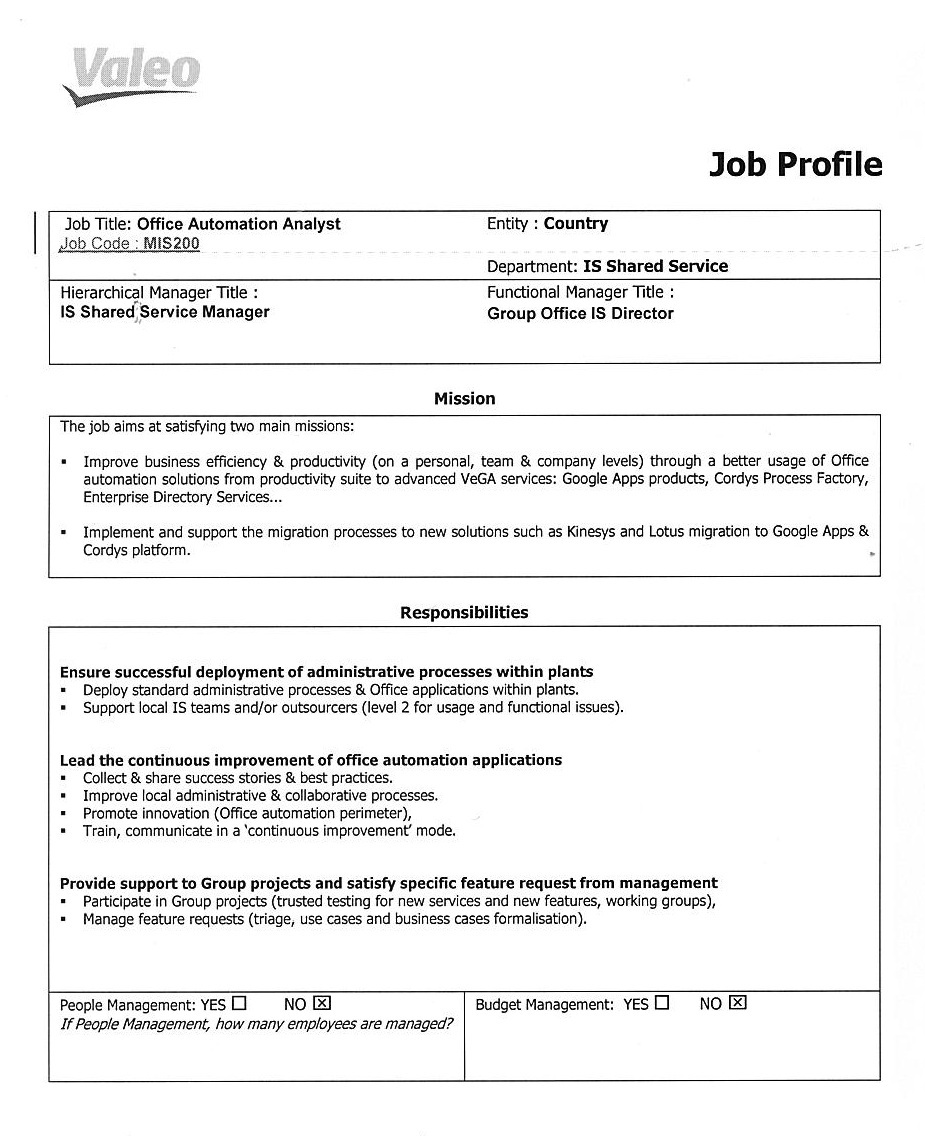
\includegraphics[height=22cm]{job_profil.jpg}
	\caption{Fiche de poste}\label{image.jobprofil} 
\end{figure} 

\clearpage


\chapter{METIS, un projet de recherche}

\section{Description du Projet de Recherche}

\textbf{Source : \url{http://metis.deltacad.fr/}}

Le projet \textbf{METIS} est un projet de recherche collaboratif impliquant deux industriels (\textbf{DeltaCAD} et \textbf{IFPEN}) et 4 laboratoires universitaires (\textbf{AMPT}, \textbf{ECN}, \textbf{UTC} et \textbf{UTT}). Ce projet est prévu pour durée de 3 ans et a débuté en octobre 2012. Le projet est subventionné par l'\textbf{ANR}, Agence Nationale de la Recherche (\url{http://www.agence-nationale-recherche.fr/}), dans le cadre du programme \textit{Modèle Numérique 2012}.

Ce projet s’intègre dans le domaine de la rétro-conception (ou \textit{Reverse Engineering} en anglais).
 
Aujourd’hui, la rétro-conception est largement utilisée dans l’industrie manufacturière afin de capitaliser des connaissances qui ne l’ont pas été jusque-là et qui deviennent aujourd’hui cruciales pour faire évoluer ses produits.
Les applications sont diverses, comme par exemple, la rétro-conception de produits existants en vue d’en modifier/combiner des composantes (cas d’IFP Energies nouvelles par exemple, qui fait de la rétro-conception de moteurs) ou alors la maintenance des produits mécaniques à très longue durée de vie (avions, navires, centrales nucléaires, plateformes pétrolières, trains…), lorsqu’il faut reconcevoir et refabriquer un composant autrefois produit soit en interne mais dont le personnel a quitté la société ou soit par un sous-traitant aujourd’hui disparu.
                                
De manière générale, les solutions commerciales présentes actuellement sur le marché proposent d’extraire les informations géométriques de l’objet afin de le reconcevoir (RAPIDFORM XOR d’Inus Technology par exemple).
Il existe également dans la littérature scientifique des approches traitant de la rétro-conception de composants ou de petits ensembles. Dans ce cas, la géométrie de l’objet est souvent obtenue par numérisation 3D ou mesure. La surface de l’objet est ainsi échantillonnée par un nuage de points et/ou un maillage surfacique. Aujourd’hui, c’est l’analyse de cette géométrie à travers un filtre de connaissances métier qui permet de retrouver les intentions initiales de conception et d’en assurer la rétro-conception.
 
Le projet \textbf{METIS} vise, quant à lui, à proposer des solutions pour la rétro-conception de grands ensembles mécaniques complexes (par le nombre de pièces et/ou leur taille) tels que des moteurs, des véhicules (ces problématiques étant au cœur des travaux d’IFP Energies nouvelles) par exemple. Dans le cadre de ces ensembles, il est délicat et peu efficace de numériser intégralement la géométrie. Par exemple, pour une automobile, relever le nuage de points de l’ensemble des pièces qui la composent serait, sinon impossible, extrêmement fastidieux. En effet, il faudrait, pour cela, démonter l’intégralité de la voiture et numériser les pièces une à une, manuellement : les systèmes de numérisation 3D automatiques de pièces dont on ne possède pas la CAO (impossibilité de faire une gamme automatique) sont très limités dès qu’il s’agit de pièces de formes complexes, la numérisation des pièces de la voiture devrait donc se faire majoritairement manuellement.
 
L’hypothèse principale portée par le projet \textbf{METIS} est que, pour la rétro-conception d’un grand ensemble mécanique complexe, les informations purement géométriques sont insuffisantes. METIS vise à proposer une solution pour intégrer l’ensemble des informations (y compris les informations géométriques) disponibles sur l’ensemble mécanique étudié afin de les traiter et d’en extraire une maquette numérique.
 
Il s’agit donc de développer des méthodologies ainsi que les outils associés qui permettront à un utilisateur de créer et maintenir dans le temps une maquette numérique sémantiquement riche et intégrant les connaissances liées à l’ensemble mécanique considéré. Cette maquette sera obtenue à partir d’informations hétérogènes, parfois incomplètes, telles que des images, des plans 2D, des nuages de points issus de numérisations 3D, des croquis, des photographies, des rapports de maintenance, des résultats de calculs…, voire même une ancienne version de la maquette numérique.

\section{Contexte scientifique}

L’objectif de METIS est de permettre la création ou la mise à jour de la maquette numérique d’un ensemble mécanique complexe existant (ex : un moteur). A partir du grand ensemble de données hétérogènes et d’une bibliothèque de composants appartenant à un domaine (composants mécaniques, mobilier, tubes, outillages, architecture), l’outil METIS permettra de déterminer automatiquement le type et le nombre de composants présents dans un ensemble mécanique complexe. Il permettra aussi de déterminer la position et l’orientation de chaque composant. Une fois que l’intégralité de la nomenclature du produit aura été déterminée et qu’une matrice de position aura été associée à chacun des composants de cette nomenclature, l’outil METIS permettra de générer la maquette numérique de ce grand ensemble mécanique. Les fonctions principales de cet environnement de rétro-conception sont les suivantes :


\begin{enumerate}
  \item Acquisition, traitement et intégration de grand volume de données, géométriques ou non, spatialement localisées : les données recueillies seront d’une telle hétérogénéité (nuages de points 3D, photographie, référence catalogue, résultats de calcul, schémas de maintenance, ancienne version de la maquette numérique etc.) qu’il faudra développer une méthodologie de triage et de mise en correspondance et de référencement innovante. Nous pourrons proposer des méta-modèles basés sur des évolutions des formalismes de cartes cognitives, de réseaux sémantiques par exemple. \\
  
  \item Méthode d’identification de composants métier dans un ensemble de données hétérogènes : il s’agira de créer d’une bibliothèque de composants caractérisés par des éléments clés (signature) permettant leur identification dans un grand volume de données. L’apport scientifique est  ici de trouver un moyen de « signer » des composants complexes et de stocker ces signatures. Elles seront établies en géométrie 2D (photographie, plan, croquis), en géométrie 3D (nuage de points) et sous toute autre forme qui pourrait être pertinente (signatures non géométriques). Cette bibliothèque permettra d’identifier, dans les données acquises précédemment, des éléments de maquette numérique associés à une signature particulière.\\
  
\clearpage

  \item Recherche, dans le grand volume de données, de la nomenclature du produit étudié ainsi que des matrices de position associées : dés qu’un composant est reconnu (identification de sa signature), le premier apport scientifique sera de le caractériser dans ses dimensions, sa position, son orientation etc. à l’aide de données géométriques et non géométriques recueillies directement dans l’ensemble de données mais aussi à l’aide de connaissances connues a priori sur le composant (ex : dépouilles si composant forgé etc.). Le second apport scientifique sera la gestion des différents niveaux de décomposition systémique lors du déroulement de METIS. En effet, l’analyse de rétro-conception peut aussi bien porter sur un système complet (ex : voiture), un sous-système (ex : ensemble moteur) ou un composant élémentaire (ex : alternateur). Les signatures et leur reconnaissance devront alors être modélisées et gérées dans ces différents niveaux systémiques qui doivent rester cohérent au fil du temps et selon la granularité de l’analyse.\\
  
  \item Génération ou modification de la maquette numérique : dés la nomenclature connue, les modèles CAO paramétrés métier associés aux différents composants pourront être :
assemblés au sein du modèle géométrique du grand ensemble étudié.
modifiés par corrélation des modèles géométriques originels et des nouveaux paramètres géométriques identifiés ou par échanges d’une partie des composants de la maquette numérique originelle. L’apport scientifique réside dans la mise en œuvre d’algorithmes et de stratégies relatifs à la manipulation de la maquette numérique soit pour la gestion de la nomenclature (ex : filtre de composants, etc.) soit pour la gestion des éléments géométriques eux-mêmes (ex : déformation, ajout sémantique, dimensionnement, etc\ldots).\\
\end{enumerate}

\clearpage


\chapter{La Reconnaissance de formes.}
\section{Qu'est ce que le reconnaissance de formes ?}

La \textbf{Reconnaissance de forme}, ou \textit{Shape Matching} en anglais, est la discipline scientifique dont l'objet d'étude est l'ensemble des méthodes et techniques permettant d'identifier un \textbf{\textit{motif}} et d'en déterminer par la suite la catégorie. C'est un domaine très lié aux méthodes dites de \textbf{Vision par Ordinateur}, ou \textit{Computer Vision} en anglais.

Ses applications sont très larges et vont de la voiture autonome qui doit pouvoir identifier un vaste ensemble de formes variées (panneaux, signalisation au sol, véhicules, personnes, animaux, obstacles ...), au contrôle qualité partiellement ou totalement automatisé.

De manière plus large, on retrouve également ce type d'algorithme en sécurité informatique ou sécurité civile pour détecter un \textit{motif de comportement anormal} : détection d'intrusion réseau, lutte anti-terrorisme \ldots

 \begin{figure}[H]
    \centering
    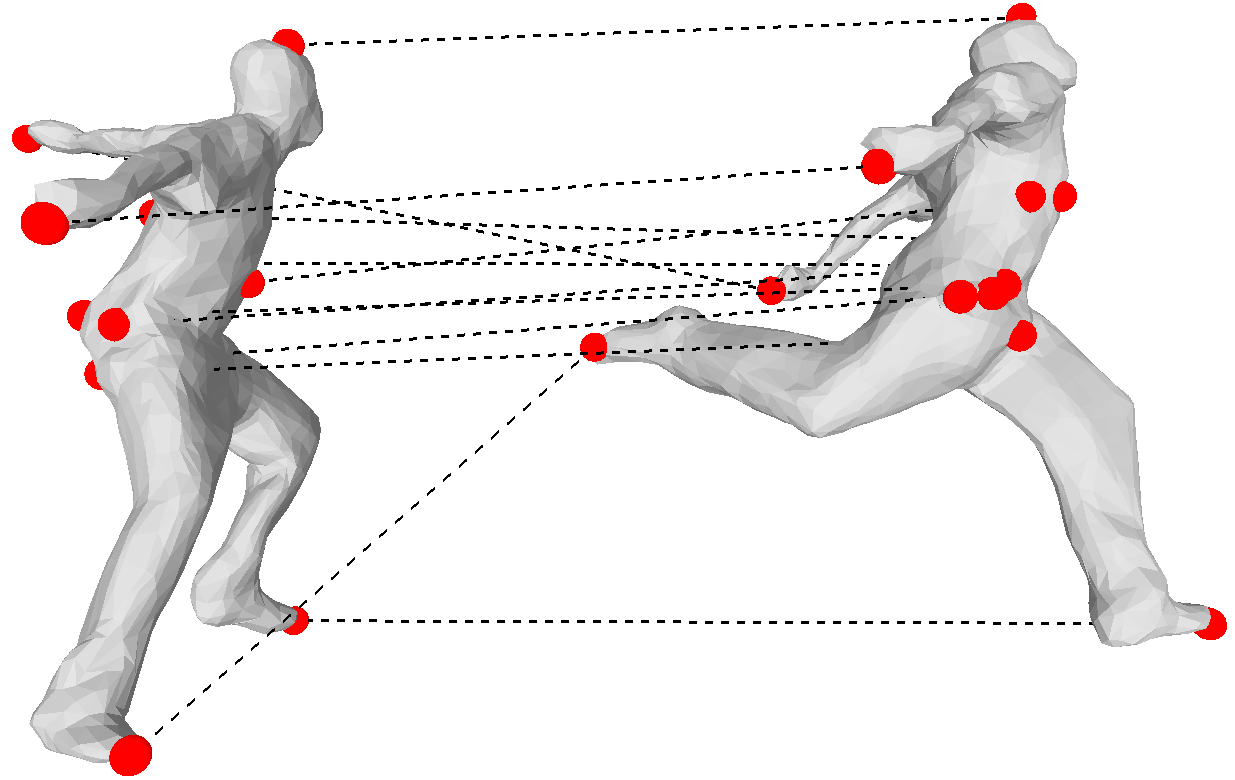
\includegraphics[height=6cm]{shapeMatching.png}
	\caption{Sortie typique d'un algorithme de reconnaissance de formes 2D/3D~\cite{shapeMatchingImg}}\label{image.shapeMatching} 
\end{figure}

 \begin{figure}[H]
    \centering
    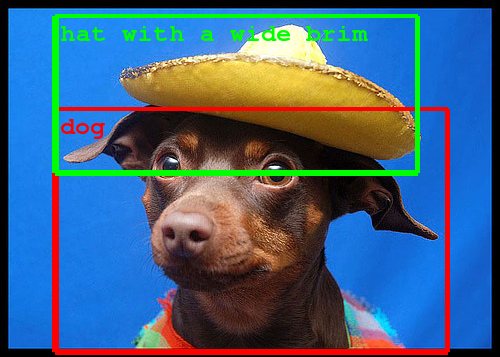
\includegraphics[height=6cm]{computerVision.png}
	\caption{Sortie typique d'un algorithme de vision par ordinateur~-~Source: \href{http://googleresearch.blogspot.fr/2014/09/building-deeper-understanding-of-images.html}{Google Research}}\label{image.computerVision} 
\end{figure}

\chapter{L'Apprentissage Automatique.}
\section{Qu'est ce que l'apprentissage automatique ?}

L' \textbf{apprentissage automatique}, ou \textit{Machine Learning} en anglais, est la discipline scientifique dont l'objectif est d'analyser une certaines quantité de données (de préférence assez grande) afin d'en déduire un modèle \textit{statistique} permettant d'\textbf{inférer} un résultat de \textbf{classification}.

On distingue principalement deux grands types d'apprentissage :
\begin{itemize}
	\item \textbf{Apprentissage Supervisé}
	\item \textbf{Apprentissage Non-Supervisé}
\end{itemize}
\vspace{3mm}

Il existe d'autres modes d'apprentissage, moins courant, sur lesquels je ne m'étendrai pas :
\begin{itemize}
	\item \textbf{Apprentissage Semi-Supervisé}
	\item \textbf{Apprentissage Par Renforcement}
	\item \ldots
\end{itemize}
\vspace{3mm}
 
Ses applications sont très larges et vont de l'\textit{analyse prévisionnelle financière}, à la \textit{détection de comportements anormaux} (Sécurité Informatique, Fraude Financière, \ldots), en passant par l'étude de la \textit{génétique} ou encore les \textit{moteurs de recommandation} comme ceux d'Amazon ou Netflix. 

 \begin{figure}[H]
    \centering
    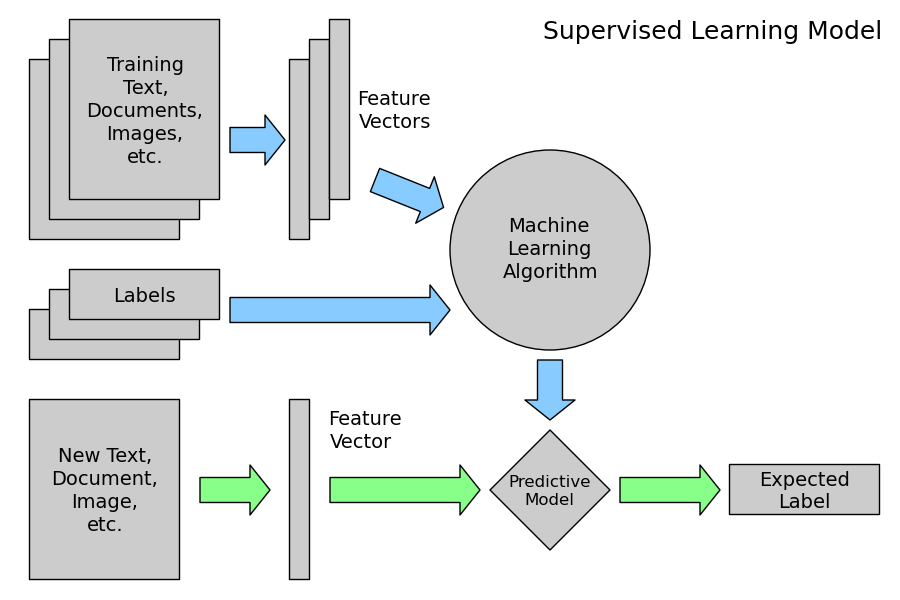
\includegraphics[height=5.5cm]{supervisedLearning.png}
	\caption{Schéma de fonctionnement d'un apprentissage supervisé~-~Source: \href{http://www.astroml.org/sklearn_tutorial/general_concepts.html\#supervised-learning-model-fit-x-y}{AstroML}}\label{image.supervisedLearning} 
\end{figure}

 \begin{figure}[H]
    \centering
    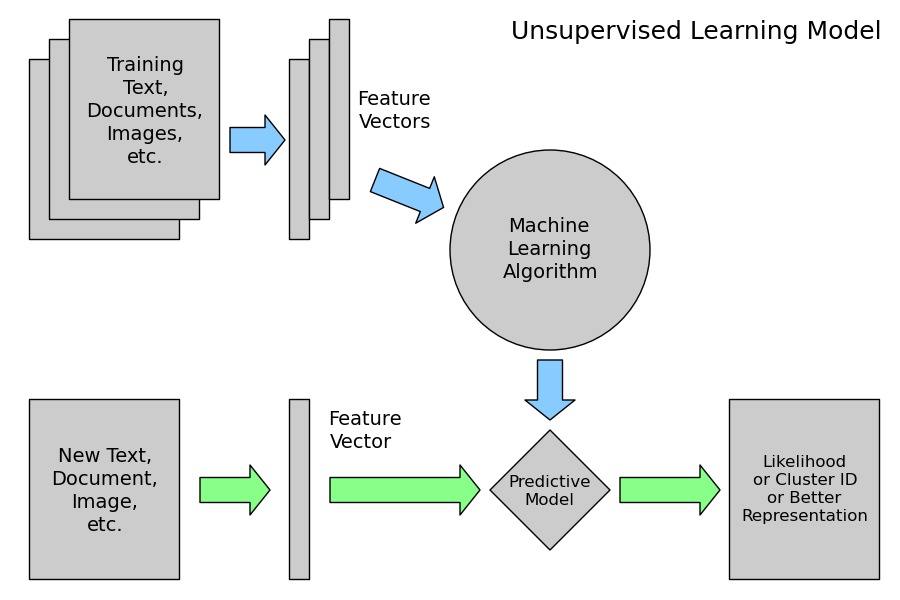
\includegraphics[height=5.5cm]{unsupervisedLearning.png}
	\caption{Schéma de fonctionnement d'un apprentissage non supervisé~-~Source: \href{http://www.astroml.org/sklearn_tutorial/general_concepts.html\#unsupervised-learning-model-fit-x}{AstroML}}\label{image.unsupervisedLearning} 
\end{figure}


\section{L'apprentissage Supervisé}

L'\textit{apprentissage supervisé} est l'une des méthodes des plus couramment utilisés dans le cadre de l'apprentissage automatique.

Pour le mettre au point, le tester et l'utiliser, nous avons besoin de trois jeux de données :

\begin{itemize}
	\item Pour la phase dite d'\textbf{apprentissage}, chaque exemple est constitué d'une paire : Un \textbf{vecteur de variables} et la \textbf{valeur de sortie} désirée.\\
	
	\item Pour la phase dite de \textbf{test}, chaque exemple est également constitué d'une paire : Un \textbf{vecteur de variables} et la \textbf{valeur de sortie} que l'algorithme devrait donner en théorie.\\ 
	En comparant la sortie théorique et celle fourni par l'algorithme sur l'ensemble du jeu de test, on obtient un indicateur de précision sur notre méthode d'apprentissage.\\
	
	\item Pour la dernière phase, dite de \textbf{production ou d'exploitation}, seul le \textbf{vecteur de variables} est connu. Nous utilisons à présent l'algorithme d'apprentissage automatique pour \textbf{inférer} le résultat de \textbf{classification}.

\end{itemize}
\vspace{3mm}

Il est important de comprendre que l'apprentissage supervisé requiert l'intervention d'un \textbf{expert} du domaine afin d'obtenir la \textit{vraie classe} de chacun des exemples des jeux de test et d'apprentissage. Cette connaissance est nécessaire à la construction des jeux de données.

\vspace{3mm}

Il existe de nombreux algorithmes permettant de mettre en place un apprentissage supervisé. On retrouve, pour les plus connus, les algorithmes suivants : 

\begin{itemize}
	\item SVM : Séparateurs à Vaste Marge (en anglais: \textit{Support Vector Machine})/\\
	
	\item KNN : Méthode des k plus proches voisins (en anglais:  K-Nearest Neighbor).\\
	
	\item Arbres de Décision.\\
	
	\item Réseaux Neuronaux (Perceptron Multicouches).\\
	
	\item Régression Linéaire.\\
	
	\item Régression Logistique.\\
	
	\item Classification naïve bayésienne.\\
	
	\item Analyse discriminante linéaire.\\
	
	\item  \ldots
	
\end{itemize}
\clearpage	
	
\section{L'apprentissage Non Supervisé}

L'\textit{apprentissage non supervisé} est un autre des modes d'apprentissage des plus couramment utilisés dans le cadre de l'apprentissage automatique.

A l'inverse de l'apprentissage supervisé, la \textit{connaissance expert} n'est pas requise. Il n'y a pas de \textit{sortie a priori}. L'objectif n'est donc pas d'inférer un résultat sur un ensemble d'étiquettes connues, mais bien de diviser un \textbf{groupe hétérogène de données}, en sous-groupes (ou \textit{clusters}) de manière à regrouper les données qui semblent les plus similaires entre elles. À l'inverse des données peu similaires devraient être dans des groupes distincts. L'\textbf{objectif} d'un algorithme d'\textit{apprentissage automatique non supervisé} est d'\textbf{extraire de manière organiser} un \textit{ensemble de connaissances} sur les données traitées.


Pour le mettre au point, le tester et l'utiliser, nous avons toujours besoin de trois jeux de données, mais qui sont cette fois ci identiques dans leur construction :

\begin{itemize}
	\item Pour la phase dite d'\textbf{apprentissage}, chaque exemple est constitué d'un \textbf{vecteur de variables}.\\
	
	\item Pour la phase dite de \textbf{test}, chaque exemple est également constitué d'un \textbf{vecteur de variables}.\\
	
	\item Pour la dernière phase, dite de \textbf{production ou d'exploitation}, toujours un ensemble d'exemples constitués d'un \textbf{vecteur de variables}.

\end{itemize}
\vspace{3mm}


Il existe de nombreux algorithmes permettant de mettre en place un apprentissage non supervisé. On retrouve, pour les plus connus, les algorithmes suivants : 

\begin{itemize}
	\item Algorithme EM : Espérance-Maximisation (en anglais: \textit{Expectation-Maximisation})/\\
	
	\item ACP : Analyse en Composantes Principales.\\
	
	\item K-moyennes (en anglais: \textit{K-Means}).\\
	
	\item Réseaux Neuronaux.\\
	
	\item  \ldots
	
\end{itemize}

\clearpage

\chapter{Les Shock Graphs}
\section*{Avant Propos}

Afin d'analyser et classifier des images 2D ou imageries 3D, il est primordial d'être capable d'extraire de ces dernières un ensemble d'informations ou "\textit{features}" qui décrivent au mieux et nous renseigne sur la nature de celle-ci.\\
On pourrait citer par exemple des critères comme la taille de la boite englobante (en anglais : \textit{bounding box}), ou encore le volume de la forme pour une pièce mécanique en 3D, en passant par la surface de cette dernière. Le critères isopérimétrique (mesure de compacité) est un excellent exemple de facteur classifiant. Il permet de discriminer, avec une bonne précision, différentes pièces mécaniques à partir de modèle 3D [M. Bruneau et al]~\cite{Bruneau2014}.

Dans le cadre de ce stage,\\
\begin{itemize}
	\item	L'accent sera porté sur une analyse d'\textbf{images en 2D}.\\
	\item	Nous cherchons à rétro-concevoir de grands ensembles mécaniques, une attention à la gestion de \textbf{grands volumes de données} doit être apportée durant tout le déroulement du projet.\\
	\item	Mettre en place une \textbf{méthode d'extraction de descripteurs} d'un fichier image (en anglais : \textit{Feature Extractor}).\\
	\item	Cette \textbf{méthode} d'extraction doit être \textbf{automatisable}. Il n'est pas envisageable, dans le cadre de notre étude, de venir renseigner à la main chacun de ces descripteurs.	
\end{itemize}
\vspace{3mm}
  

\section{Les Shock Graphs}

\subsection{État de l'art et méthodes d'extraction de descripteurs.}

Suite à trois semaines d'analyse de la littérature scientifique, il en est ressorti plusieurs méthodes qui pourraient satisfaire nos besoins. La plupart de ces méthodes sont directement dérivées du domaine de la \textbf{Vision par Ordinateur}.

J'ai testé plusieurs méthodes basées sur différentes approches du problèmes :
\begin{itemize}
	\item Filtre de Canny
	\item Algorithme SURF
	\item Réseaux de Convolutions
	\item Shock Graphs
	\item \ldots
\end{itemize}
\vspace{3mm}

\begin{figure}[H]
    \centering
    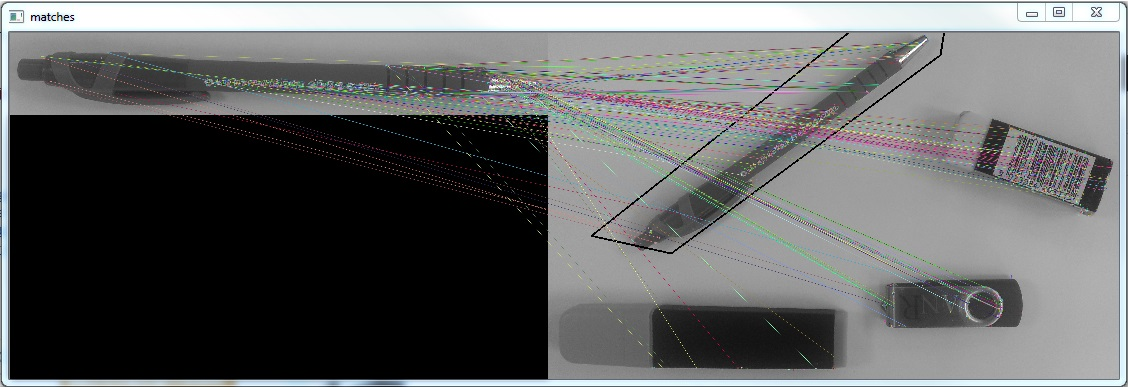
\includegraphics[height=5.5cm]{CannySurfClean.jpg}
	\caption{Output d'un test avec l'algorithme SURF, cible totalement visible} 
\end{figure}
\vspace{-6mm}

\begin{figure}[H]
    \centering
    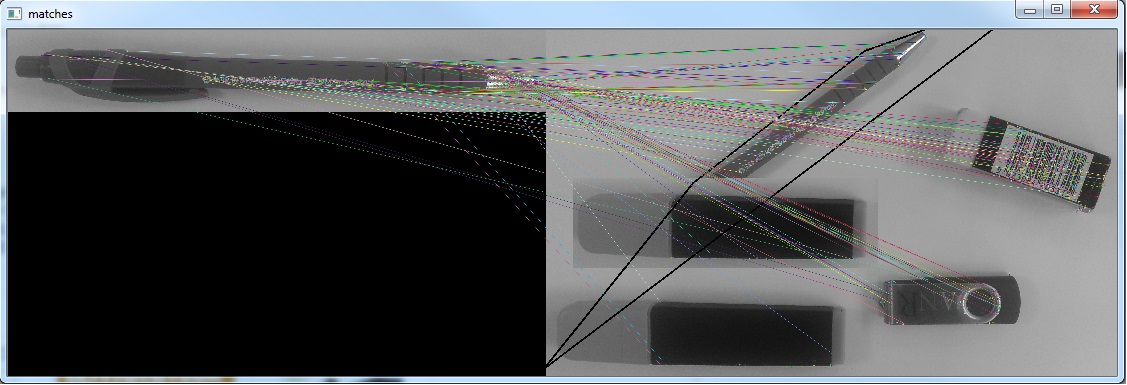
\includegraphics[height=5.5cm]{CannySurfPartiallyMasked.jpg}
	\caption{Output d'un test avec l'algorithme SURF, cible partiellement visible}\label{image.CannySurfPartiallyMasked} 
\end{figure}
\vspace{-6mm}

Il apparait que l'algorithme SURF manque de précision et vient \textit{accrocher} tous les objets de la scène. D'avantages d'investigations ont mis en évidence que l'algorithme étant basé sur la détection de points d'intérêt n'est pas capable d'apprendre une forme mais uniquement les détails d'un objet spécifique. Raisons qui font de l'algorithme SURF un \textbf{mauvais candidat} pour notre étude.

\clearpage
\subsection{Tests préliminaires sur le fonctionnement des Shock Graphs}

Suite à mes recherches bibliographiques, j'ai pu mettre en évidence les travaux sur les Shock Graphs. Ce sont des graphs qui décrivent une forme binaire 2D (Blanche ou Noire, pas de gris) par le biais d'un \textit{squelette} ou \textit{axe médian de Blum}. Leur fonctionnement et leur utilisation est décrite par [K. Siddiqi et al]~\cite{Siddiqi1999}. Un démonstrateur scientifique ainsi qu'une méthode de comparaison de ces graphs a été mise au point par [D. Macrini et al]~\cite{Macrini2002} dans le cadre de son mémoire de master.

À partir de ces travaux, j'ai pu mettre sur pied assez rapidement un test mettant en évidence la pertinence de la méthode relative à notre usage. Et je dois bien admettre avoir été bluffé par la précision de cette méthode. Sentiment qui semble avoir partagé autour de moi.

J'ai créé donc pour le test un jeu de données d'apprentissage et un jeu de test. Chacun contenant un ensemble de vues des pièces mécaniques suivantes:
\begin{itemize}
	\item 	Piston
	\item	Bielle
	\item	Assemblage Piston/Bielle
	\item	Roue dentée
\end{itemize}
\vspace{5mm}

\begin{figure}[H]
    \centering
    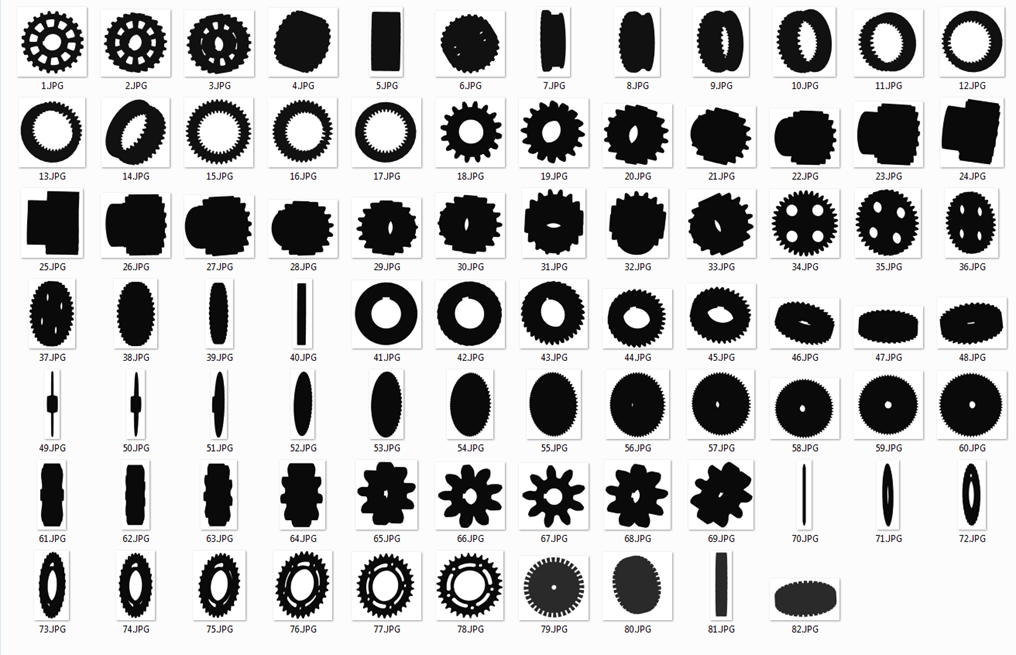
\includegraphics[height=7cm]{datasetShock.png}
	\caption{Exemple de base de connaissances sur les roues dentées, en vue du test des Shock Graphs}\label{image.ShockGearDataset} 
\end{figure}
\vspace{-4mm}

\begin{figure}[H]
    \centering
    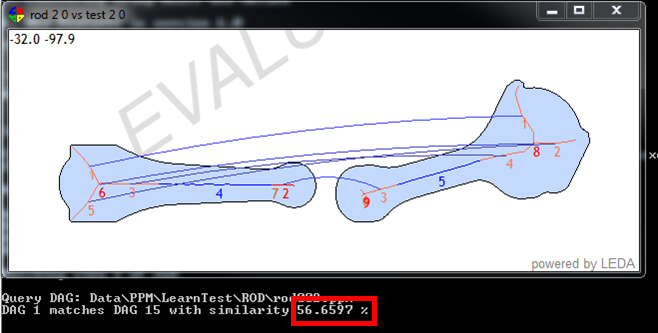
\includegraphics[height=5.5cm]{ShockTest1.png}
	\caption{Output d'un test utilisant les Shock Graphs, \textbf{56.6597\% de match}.}\label{image.ShockTest1} 
\end{figure}


\clearpage

\subsection{Principe de fonctionnement des Shock Graphs.}

Lotus Notes (solution logicielle développée par \textbf{IBM}) et Cordys Process Factory (solution Cloud développée \textbf{Open~Text}) ont un objectif commun : proposer une réponse au  besoin de ``\textit{Business Processing}" au sein d'une entreprise.

Cependant elles diffèrent sur l'architecture (serveurs et réseau) nécessaire à son fonctionnement :

\begin{itemize}
		\item Lotus Notes se base sur une architecture type logiciel Client / logiciel Serveur, les serveurs sont inter-connectés entre eux et ``\textit{répliquent}" certaines de leur données à intervalle de temps régulier. Ce fonctionnement est coûteux , il demande une infrastructure imposante ainsi qu'une administration au jour le jour. \\
		Plus gênant, comme il est difficile d'avoir une vue d'ensemble du système actuel, la quantité d'application dupliquée ne cesse d'augmenter, ce qui induit des coûts de fonctionnement de plus en plus élevés.\\

	\item Cordys Process Factory propose une réponse orientée ``\textit{Cloud Computing}" à ces problématiques, nous pouvons donc faire \textit{abstraction} de l'architecture réseau et serveur nécessaire à son fonctionnement (gérée par le fournisseur du service). La plateforme est accessible via un navigateur web, nul besoin de paramétrer son ordinateur ou d'installer un quelconque logiciel.\\
	Le choix de Cordys Process Factory est donc cohérent avec la politique actuelle du groupe Valeo qui cherche à \emph{externaliser} la gestion de la partie infrastructure et l'administration des diverses solutions informatiques.\\
	\end{itemize}


Valeo a fait le choix de se baser en grande partie sur la suite Google Apps pour un maximum de services et besoins bureautiques. Ainsi nous utilisons de manière non exclusive: 

	\begin{itemize}
		\item Gmail
		\item Google Drive
		\item Google Apps (SpreadSheet, Docs, Presentation, Scripts, Sites)
		\item Google Agenda 
		\item Google AppEngine
	\end{itemize}

En complément nous utilisons un LDAP, commun à tous les sites Valeo du monde, interfacé avec la suite applicative de \textbf{Google}. Valeo appelle cet ensemble de systèmes inter-opérants  : VeGA \textit{(Valeo empowered by Google Apps)}.

\textbf{Et \textit{Cordys Process Factory} dans tout ça ?}

Fort de sa position de partenaire \emph{Google Entreprise}, Cordys Process Factory permet une inter-connection aux services Google Apps  et le LDAP de Valeo : \textit{l'Entreprise Directory}.\\
Ainsi les \textit{Businness Process} et \textit{Businness Workflows} peuvent s'appuyer sur les services et applications déjà en place chez Valeo afin de réduire les coûts de mise en place et de développement.

\clearpage
\clearpage

\chapter{Shape Learner - Plugin METIS}
\section{ShapeLearner - Un plugin de signature}

METIS, en plus d'être un projet de recherche est également le nom du logiciel qui lui est associé. Ce dernier est programmé en JAVA. Il propose une interface à laquelle on peut venir adjoindre de multiples plugins de \textbf{signature}.

Ces derniers se doivent de répondre aux spécifications suivantes :
\begin{itemize}
	\item Être compilé sous forme d'une librairie DLL ou utiliser le langage JAVA.
	\item Exposer une fonction de signature en contexte : \textit{Signature SignInContext(Context);}
	\item Exposer une fonction de comparaison en contexte : \textit{Output MatchInContext(Signature, Context);}
\end{itemize}

\subsection{L'objectif du plugin ShapeLearner}

L'objectif de ce plugin est d'identifier la \textbf{classe} d'un composant mécanique ou d'un assemblage mécanique et ce en prenant en entrée une image 2D de l'objet. Celui-ci doit être le plus robuste possible aux effets d'échelle et à l'angle de prise de vue de l'objet.

Ainsi le plugin doit être capable de donner en sortie le type de pièce ou d'assemblage donné en entrée. \textit{\textbf{Exemple:} Bielle, Piston, Vilebrequin, ...}.

Il est envisageable que l'algorithme retourne soit un seul résultat soit un nombre restreint de résultats avec leur indice de confiance \textit{(par exemple les 3 meilleurs)}. Ce choix pouvant être, par exemple, contrôlé par l'utilisateur. 

\subsection{Le plugin C++ ShapeLearner}

En se basant sur le travail effectué par D. Macrini et al.~\cite{Macrini2002}, nous avons décidé d'adapter le démonstrateur fonctionnel à nos besoins. En effet ce dernier a été publié sous licence Open Source, et a été entièrement programmé en C++.

Dans le soucis de faciliter l'intégration du démonstrateur à notre plugin, nous avons fais le choix d'utiliser nous aussi le langage C++.

\subsubsection{L'architecture logicielle}

Un des points centraux de l'architecture fut de permettre l'utilisation \textbf{\textit{multi-thread}} du démonstrateur fonctionnel mis au point par  D. Macrini et al.~\cite{Macrini2002}. 

Le plugin se compose lui même de plusieurs modules (les modules sont listés en partant de la couche la plus basse jusqu'à la couche supérieure qui est l'interface DLL du plugin) :

\begin{itemize}	
	\item \textbf{Module StandardException: } Ce module a pour rôle de proposer une classe d'exception standard et enrichie pour tout le plugin. Chaque exception générée au sein du programme est gérée de manière unique grâce à cette classe.\\

	\item \textbf{Module CLogger: }``Concurrent Logger'' a pour tâche de réaliser la totalité des actions de \textbf{\textit{logging}} au sein de l'application. Ce module présente une interface entièrement \textbf{\textit{thread-safe}}.\\
	Ce dernier pour notre cas génère quatre fichiers :
	\begin{itemize}
		\item ShapeLearner.Core.log
		\item ShapeLearner.DB.log
		\item ShapeLearner.Error.log
		\item ShapeLearner.Exec.log
	\end{itemize}
	\vspace{3mm}
	
	 \item \textbf{Module GraphDBLib: }Ce module sert de moteur de sauvegarde et de chargement des données depuis et vers les bases de données PostgresSQL associées. Il a été entièrement programmé pour permettre jusqu'à 200 threads concurrents. Il propose une structure objet classique de Graph (Noeuds, Arêtes, ...). Ce dernier gère de manière totalement automatique, transparente et optimisée les interactions avec la base de données. Il est important de préciser que ce module présente deux interfaces. L'une en utilisation classique, l'autre de type SDK permettant de définir des attributs spécifiques ou sous-classes pour chacune des structures classiques du Graph. L'objectif étant de ne pas rendre dépendant le module de la structure spécifique du ShockGraph ou d'un quelconque autre type de Graph. Ce module utilise les deux modules cités plus haut.\\
	 
	 \item \textbf{Module DAGMatcherLib: } Reprise du démonstrateur scientifique de D. Macrini et al.~\cite{Macrini2002}. Modifié afin d'en améliorer les performances, et de permettre l'utilisation multithread. C'est ce dernier qui génère la \textbf{signature} de notre plugin ! C'est le \textbf{cœur} du plugin \textbf{\textit{ShapeLearner}}. Celui se branche directement sur les modules précédents afin de logger les divers évènements lors de la génération de la signature et de sauvegarder le résultat en base de données.\\
	 
	 \item \textbf{Module ShapeLearnerLib: } Module chef d'orchestre, il coordonne les actions et lance la génération des signatures de manière concurrente grâce à l'utilisation d'une threadPool. Ce module est l'unique point d'entrée du plugin. Ce dernier est compilé sous forme de librairie statique (.lib sous windows). C'est ce module qui expose la totalité des fonctionnalités du plugin à destination de pour tout projet visant à la création d'une librairie dynamique ou d'un exécutable utilisant ce plugin.\\
	 
	 \item \textbf{Module ShapeLearnerDLL: } Ce module présente les fonctionnalités du plugin ShapeLearner\- via une interface librairie dynamique (.dll sur windows). Aucune fonctionnalité n'est implémentée dans ce module, il ne fait que transmettre les opérations au module ShapeLearnerLib.\\
\end{itemize} 

\clearpage

Une réel soucis de modularité et non dépendance ascendante des modules entre eux a été la base de notre réflexion. Nous voulions que chaque module du plugin puisse avoir un maximum de sens en dehors de tout contexte. Le but étant de pouvoir réutiliser chacun de ces modules dans une application future si l'occasion se présente. 

Les relations d'interdépendance sont donc à limiter autant que possible. Cependant une relation de dépendance \textbf{\textit{top-down}} est tout à fait possible et même nécessaire. Ainsi le plugin est construit en couches successives. Chaque couche peut interagir avec les couches inférieures, jamais supérieures ou de même niveau.
\vspace{-1cm}

 \begin{figure}[H]
    \centering
    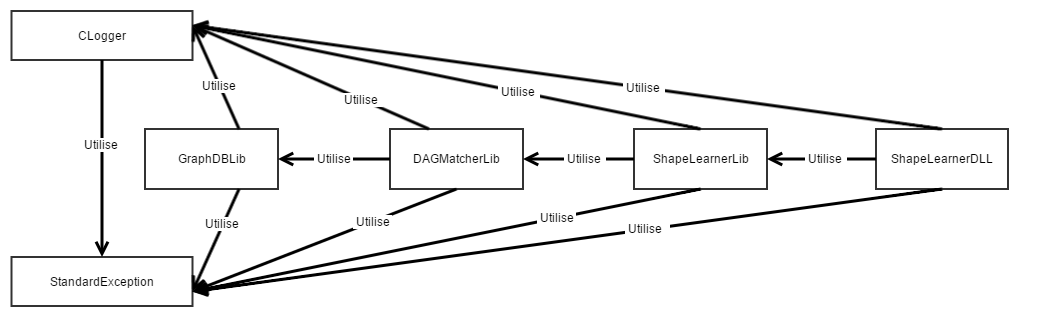
\includegraphics[angle=90,origin=c,height=12.8cm]{shapelearnerplugin_architecture.png}
	\caption{Schéma de l'architecture interne du plugin C++ : ShapeLearner}\label{image.archiShapeLearner} 
\end{figure}

\clearpage

 \begin{figure}[H]
    \centering
    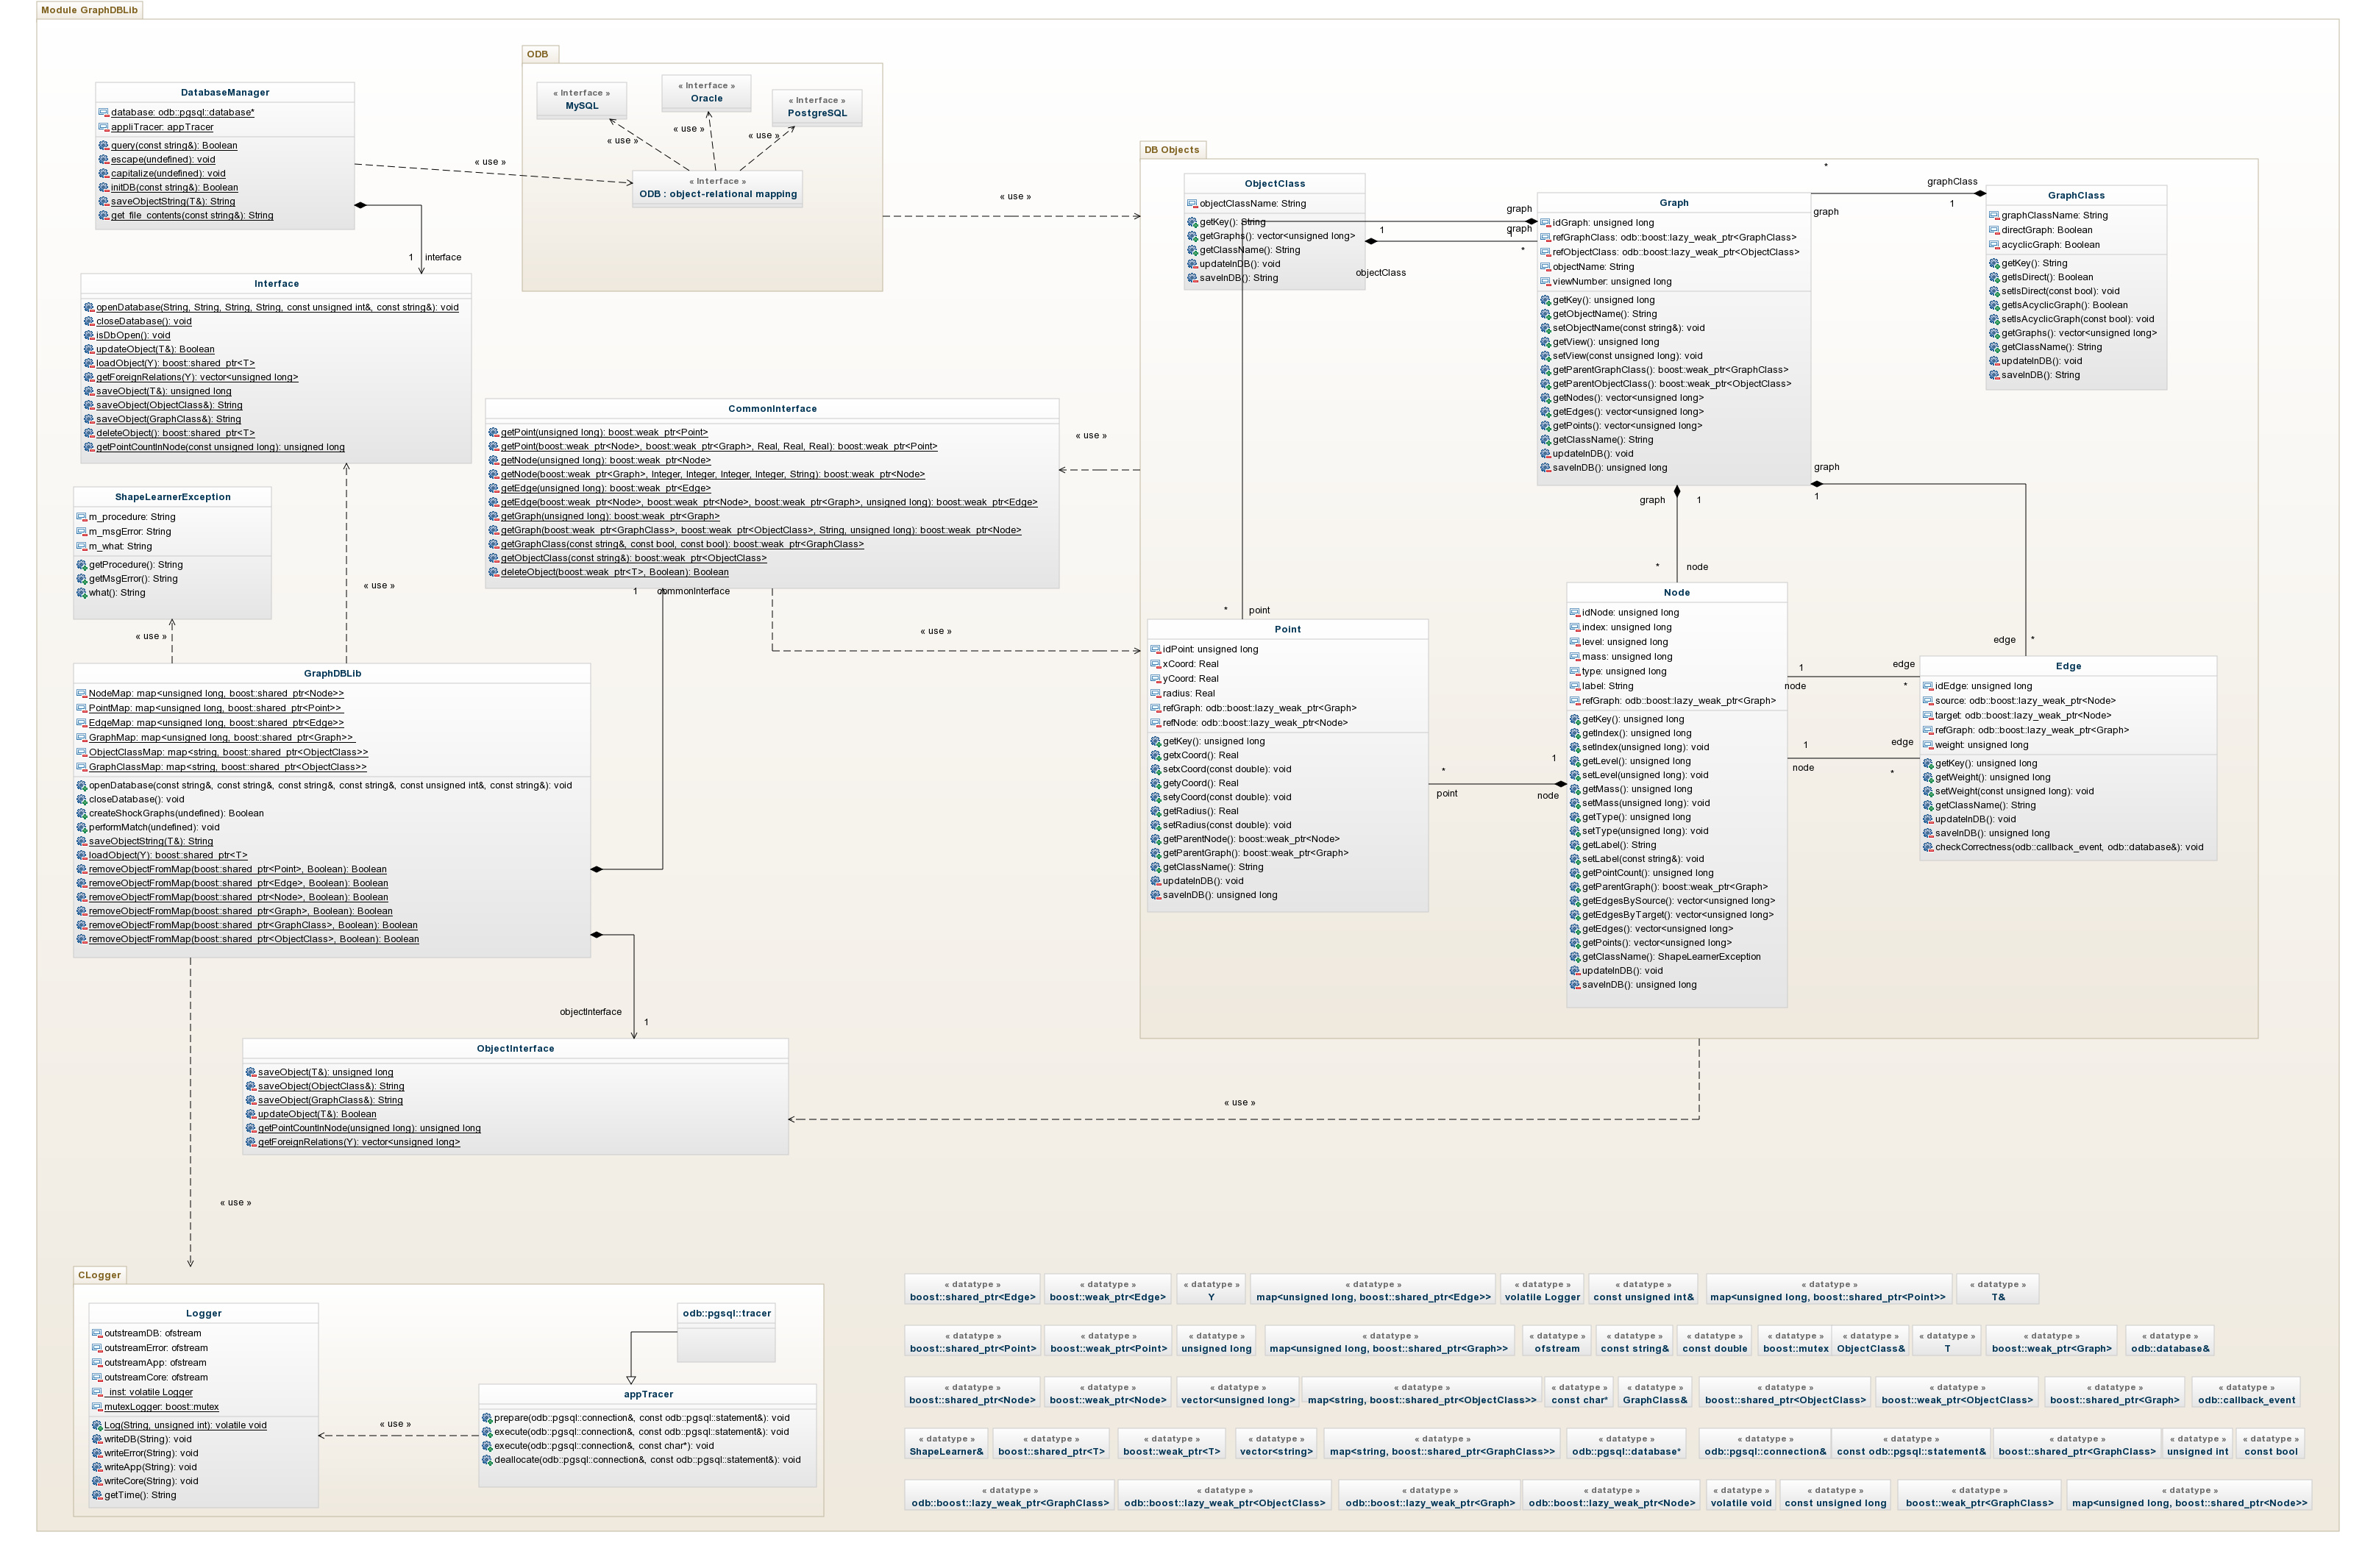
\includegraphics[angle=90,origin=c,height=19cm]{ShapeLearner_UML.jpg}
	\caption{Diagramme UML simplifié présentant le principe de l'architecture du module GraphDBLib\-. Il a pour objectif d'expliquer de manière simple les interactions possibles au sein du module GraphDBLib. La totalité des liens, relations et associations n'est donc pas représentée.}\label{image.UMLGraphDBLib} 
\end{figure}

\subsection{Portage sur le cloud Amazon : AWS}

\subsubsection{L'application web RESTful - ShapeLearnerAPI}

Le plugin est plutôt intensif en calcul, ajoutons à cela les nombreuses interactions avec la base de données. Cela donne un résultat manquant de souplesse, fortement dépendant de la qualité du réseau de l'utilisateur et de la puissance de la machine hôte.\\
J'ai eu l'occasion, pendant ce stage, de tester les nombreuses opportunités offertes par le \textbf{cloud Amazon : AWS}.
J'ai ainsi standardisé le processus d'installation et automatisé la majeure partie. Le front-end de l'application a été codé en Python, j'ai choisi d'utiliser le framework web : Bottle.py (\url{http://bottlepy.org/}) afin d'exposer l'ensemble des fonctionnalités du plugin via une interface de type API RESTful.

Le cloud Amazon permet de lancer de manière automatique suffisamment d'instances identiquement paramétrées afin de supporter la charge sur l'application. Un \textit{load-balancer} permet de répartir les demandes à travers les différentes instances actives.

\subsubsection{Le plugin ShapeLearner}

Un plugin Java a été élaboré afin d'aller requêter les services exposés par l'Application Web: ShapeLearnerAPI\-. Chacune des fonctionnalités étant un appel réseau à l'adresse du service correspondant. 

Le \textit{load-balancer} se charge à ce niveau de répartir la charge des calculs à travers les différentes instances actives de l'API. C'est également lui qui fait le choix de lancer ou d'éteindre des instances en fonction de la charge (selon des règles qui sont définies en amont).

\clearpage

\subsubsection{Docker - La plateforme de conteneurisation}

Toujours dans l'objectif d'accélérer le processus de développement et de standardiser la mise en production, nous avons fais le choix d'utiliser Docker (\url{https://www.docker.com/}) qui est un logiciel, disponible sous distribution Linux et très bientôt il semblerait sur Windows également. Ce dernier permet la création d'environnement standardisés, épurés, légers, prêts à l'utilisation.


\begin{chapquote}
{Site Internet de Docker, \url{https://www.docker.com/}}
\begin{verse}
"Docker is an open platform for building, shipping and running distributed applications. It gives programmers, development teams and operations engineers the common toolbox they need to take advantage of the distributed and networked nature of modern applications."\\
\vspace{3mm}
"Docker est une plateforme ouverte pour créer, distribuer, et lancer des applications. Docker propose aux programmeurs, aux équipes de développement, et aux ingénieurs d'exploitation une boite à outils commune permettant de tirer avantage de la nature distribuée et en réseau des applications modernes."
\end{verse}
\end{chapquote}

J'ai utilisé Docker en particulier pour le déploiement des deux bases de données PostgreSQL:
\begin{itemize}
	\item PostgreSQL 1: Base de connaissances
	\item PostgreSQL 2: Base de production
\end{itemize}
\vspace{3mm}

\subsubsection{Optimisation de la base données}

Afin d'optimiser les requêtes en lecture sur la base de données utilisées par le module PredictionAPI (voir \nameref{subsec:PredictionAPI}), je me suis posé la question du type de stockage optimal au sein de la base de données.

En effet, historiquement, les données sont stockées en ligne. Chaque enregistrement représente un ou plusieurs blocs mémoires qui sont, si possible, à la suite sur les disques. Le problème étant que lorsqu'il faut lire peu de colonnes et grande quantité de lignes, il est alors nécessaire de lire quasiment l'intégralité des blocs mémoires de la table. Pour peu qu'il y ait quelques dizaines de million de lignes, les disques classiques risquent bien de montrer de très faibles performances. La RAM va de son côté réaliser de très nombreux \textbf{\textit{swap}}, bref une situation très problématique.

C'est ainsi que de nombreux éditeurs de base de données analytiques mettent au point de nouveaux moteurs permettant le stockage des données en colonnes.

Cependant ce dernier provoque le problème inverse: \textit{peu de lignes et beaucoup de colonnes}. On peut cependant penser que ce problème est plus rare, et qu'on a rarement quelques dizaines de million de colonnes.

Cependant, afin de maximiser l'optimisation, certains éditeurs de base de données ont mis au point des moteurs hybrides permettant à la fois le stockage en colonne et en ligne de manière simultanée, choisissant le meilleur système de stockage en fonction de la requête. On pourrait citer par exemple : SAP Hana.

J'ai personnellement utilisé le moteur \textbf{cstore\_fdw} développé par citusdata \url{https://www.citusdata.com/citus-products/cstore-fdw}, un plugin pour PostgreSQL. J'ai réussi à le paramétrer afin de permettre le stockage en colonne et en ligne. Seulement n'ayant pas le temps de réécrire un optimiseur de requête pour le moteur de PostgreSQL, je laisse le soin à l'utilisateur de choisir le stockage idéal pour sa requête. L'utilisation du mot clé SQL "\textit{Explain}" peut donner une excellente indication pour faire son choix.


\subsubsection{ShapeLearner - PredictionAPI}
\label{subsec:PredictionAPI}

Afin de ne pas comparer chaque pièce à l'ensemble des pièces de la base de connaissance, il a fallu trouver un moyen de trouver les "plus probables" sans effectuer pour autant la comparaison des graphs qui est assez intensive en calculs.\\

J'ai donc utilisé Docker pour déployer un environnement Python afin de tester divers algorithmes d'apprentissage automatique supervisé.

 \begin{figure}[H]
    \centering
    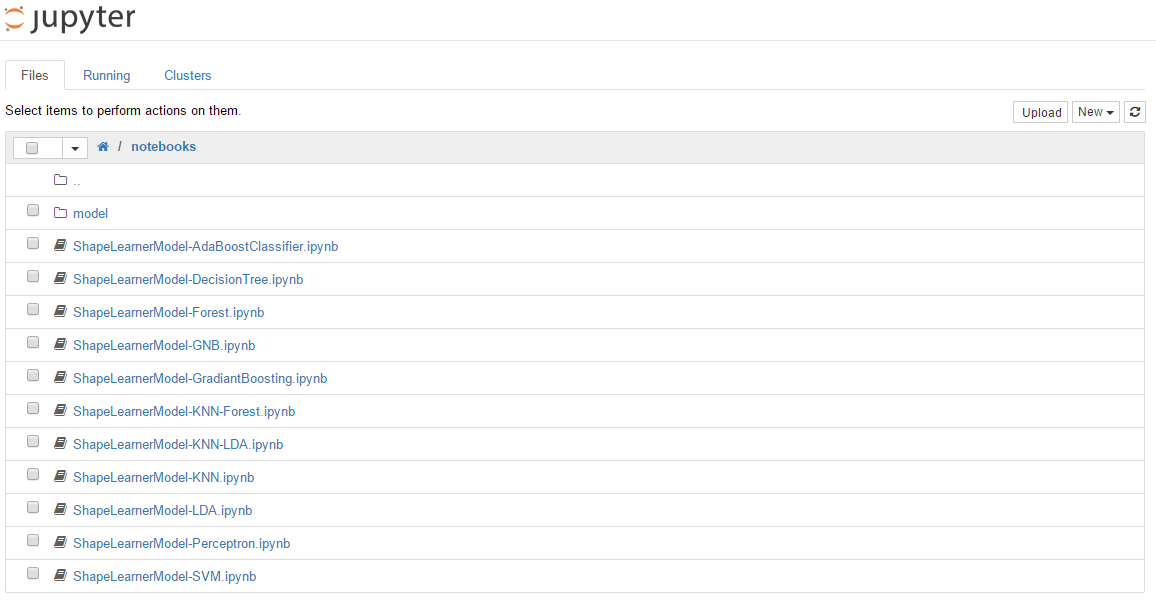
\includegraphics[width=18cm]{machineLearningAlgorithms.png}
	\caption{La totalité des algorithmes d'apprentissage automatique testés.}\label{image.MLListe} 
\end{figure}

Je regrette cependant ne pas avoir pu passer suffisamment de temps pour explorer toutes les pistes que j'avais pour améliorer le pourcentage de réussite. J'ai dû me contenter du résultat certes satisfaisant mais pouvant être très certainement amélioré.

L'algorithme donnant le meilleur résultat est le celui des \textit{k-plus-proches-voisins ou KNN (K-Nearest-Neighbors)} de la librairie Python : \textbf{\textit{Scikit-learn}}. J'ai obtenue le meilleur résultat en prenant les paramètres suivants :

\begin{itemize}
	\item \textbf{neighbors =}  53
	\item \textbf{weights =}  distance
	\item autres paramètres = valeur par défaut
\end{itemize}

\begin{center}
\textbf{On obtient un résultat de classification quasiment instantané avec une précision de l'ordre de 50\%.}
\end{center}

La valeur élevée du nombre de voisins peut s'expliquer par le fait que chaque pièce de la base de connaissance est représentée par environ 70 photos selon un grand nombre d'angles. Un nombre faible de voisins correspondant serait donc peu pertinent.

Dans la même idée, les poids des plus proches voisins ne sont pas uniformes mais fonction de l'inverse de la distance afin de fortement privilégier une grande ressemblance au détriment d'une faible correspondance.

Les données d'apprentissage qui sont en entrée de l'algorithme sont les \textit{\textbf{métadonnées}} des ShockGraphs générés. Par exemple, le nombre de nœuds, le nombre d'arêtes, le nombre d'arêtes par nœud, la taille de la boite englobante de l'objet ...

\subsubsection{ShapeLearner - PredictionAPI - Utilité ?}

La prédictionAPI sert de \textbf{filtre} afin de réduire le champs des possibles. Ainsi au lieux de comparer la pièce candidate à la totalité des pièces en base de connaissance, nous pouvons uniquement la comparer aux N-plus-probables. Ce qui aura pour effet de considérablement raccourcir le temps de traitement. L'objectif de la PredictionAPI n'est pas de fournir un résultat absolu mais d'éliminer les classes d'objets qui semblent sans rapport.

\subsubsection{ShapeLearner - PredictionAPI - Comment améliorer la précision ?}

Il est plus qu'envisageable qu'une étude plus approfondie aurait pu permettre de meilleurs résultats. J'aurais par exemple voulu avoir le temps de tester les réseaux de neurones multi-couches de manière plus poussée. Il semblerait que ces derniers soit particulièrement efficaces dans le domaine de la vision par ordinateur.

J'aurais également voulu avoir un peu plus de temps pour tester diverses combinaisons de modèle d'apprentissage. Pratique qui semble considérablement améliorer les résultats.

\subsection{Résultat finaux - ShapeLearnerAPI}

A l'heure où j'écris ce rapport, nous n'avons pas encore été en mesure d'effectuer les test finaux d'exécution du plugin ShapeLearnerAPI et de comparaison avec une base de test établie correctement. Cependant nous pouvons avancer des résultats très encourageant. La méthode affiche une précision qui avoisine les 70\% de réussite en temps suffisamment court pour être acceptable.

\subsection{Schéma de l'API}

 \begin{figure}[H]
    \centering
    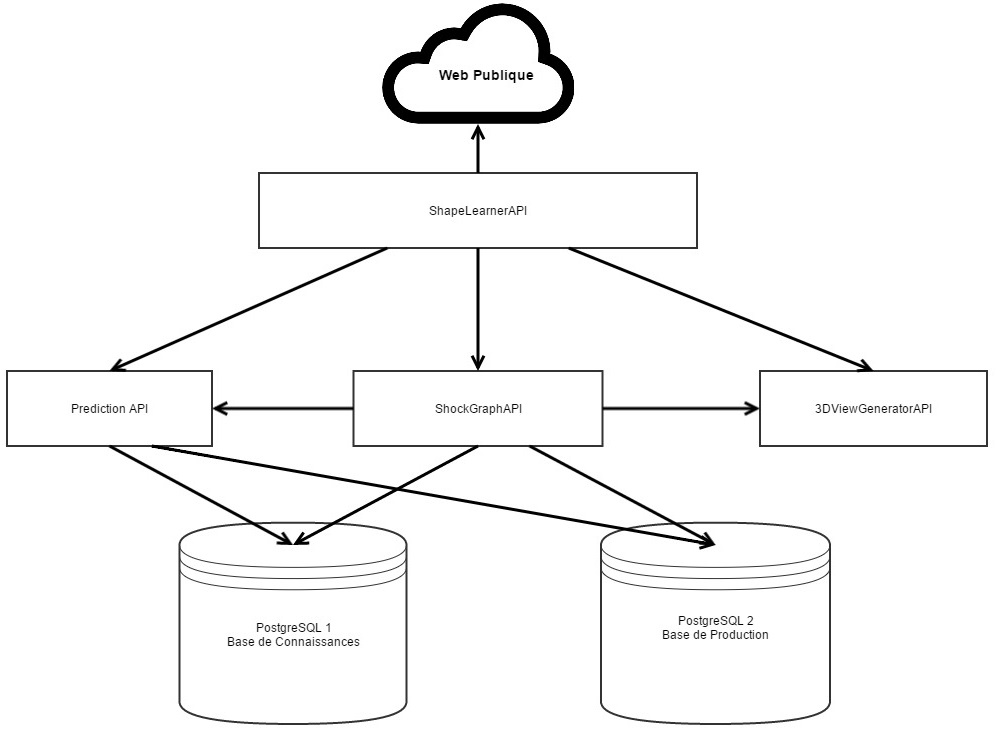
\includegraphics[width=18.7cm]{shapelearnerapi.jpg}
	\caption{Schéma interne côté serveur de ShapeLearnerAPI.}\label{image.ShapeAPIScheme} 
\end{figure}

\clearpage

\chapter{Conclusion}

C'est avec plaisir que, maintenant, je peux regarder en arrière, rire de mes erreurs, sourire de mes nombreuses questions mais surtout être satisfait du chemin parcouru.

Les nombreux problèmes qui se sont posés à moi m'ont forcé à toujours aller plus loin dans mes raisonnements et mes recherches, à trouver \textit{la parade} ou \textit{l'astuce} qui fera que \textit{cette fois-ci, ça marchera}.

Ce fut également un moment où j'ai pu tiré profit de l'enseignement reçu à l'UTC ainsi que lors de mes deux Erasmus à Vienne et Hamburg. Ce fut également l'occasion de mettre en difficulté mes connaissances afin de consolider mes acquis.

J'ai eu l'occasion d'acquérir une première expérience du monde de la recherche avec un projet concret : METIS. Mais également l'opportunité de découvrir un cas concret d'utilisation de la Vision par Ordinateur et de l'apprentissage automatique. Ce fut également une chance unique de découvrir le monde du développement logiciel et le développement de services basés sur le cloud mais également d'entrevoir les problématiques et challenges de la rétro-conception de grands ensembles mécaniques.

J'en profite, encore une fois, pour remercier tout ceux qui ont participé au bon déroulement de ce stage. 

Je ne saurais faire la liste de tout ce que j'ai pu apprendre, cette expérience me sera très utile pour la suite de mon projet professionnel: Réaliser une thèse sous la direction de M. Durupt à l'UTC et la codirection de M. Kiritsis à l'EPFL. Il est un premier élan dans le monde de la recherche et un point final à mon cursus d'ingénieur.

% Pour finir l'interligne de 1,5
%\end{onehalfspace}

%----------------------------------------
% Pour la bibliographie
%----------------------------------------
% Citer tous les ouvrages/références
\nocite{*}

\bibliography{IEEEabrv,biblio}

\printindex

\appendix

\pagebreak

\chapter*{Rédaction du Rapport en langage LaTeX}
\markboth{Langage LaTeX}{}
\addcontentsline{toc}{chapter}{Rédaction du Rapport en langage LaTeX}
Ce rapport a été entièrement rédigé en \href{http://fr.wikipedia.org/wiki/LaTeX}{\textbf{LaTeX}}. 

Les sources sont disponibles et téléchargeables sur Github à l'adresse suivante :\\
\textbf{\url{https://github.com/DEKHTIARJonathan/Rapport-TN10}}

\end{document}
